\section{Metodologia}

O experimento foi divido em duas partes principais, primeiro com o ensaio do motor de indução com rotor em vazio e depois o ensaio do motor com rotor bloqueado. Utilizou-se o motor cuja placa está apresentada na figura \ref{placa} e o motor completo está na figura \ref{motor}. Também foi utilizado o multimedidor para fornecer medições de grandezas elétricas (tensão, corrente, potência, etc.) que está disposto na figura \ref{multimedidor}. Um variac foi utilizado para fornecer tensão variável aos enrolamentos do estator do motor e este está disposto na figura \ref{variac}. Vale destacar que o fornecimento de tensões trifásicas do variac estava um pouco desequilibrada. A prática foi montada como disposto na figura \ref{pratica}



\begin{figure}[h!]
\centering
    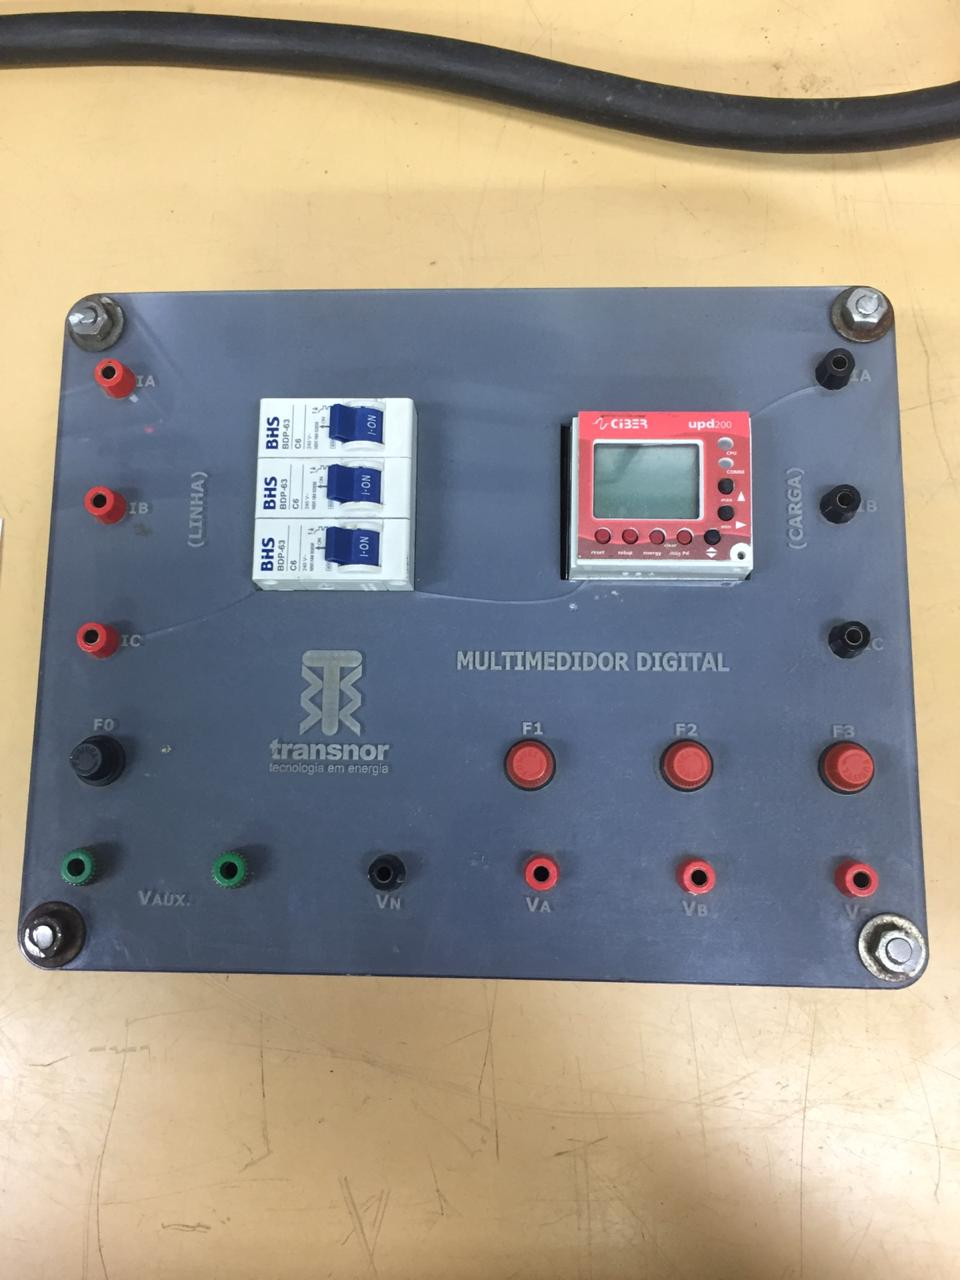
\includegraphics[width=5cm]{images/mult.jpeg}  
\caption{Multimedidor.}
\label{multimedidor} 
\end{figure}

\begin{figure}[h!]
\centering
    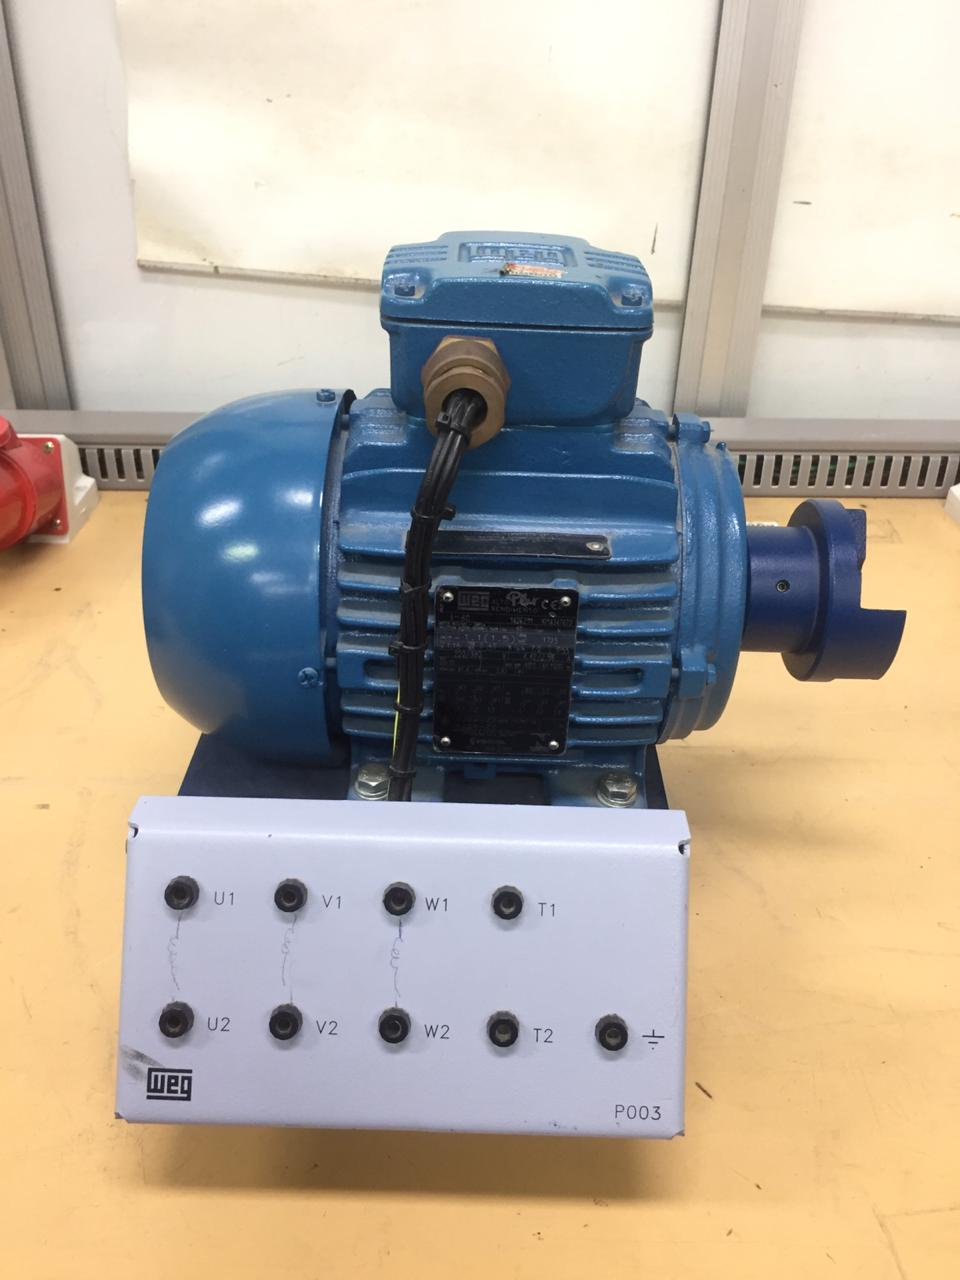
\includegraphics[width=5cm]{images/motor.jpeg}  
\caption{Motor.}
\label{motor} 
\end{figure}

\begin{figure}[h!]
\centering
    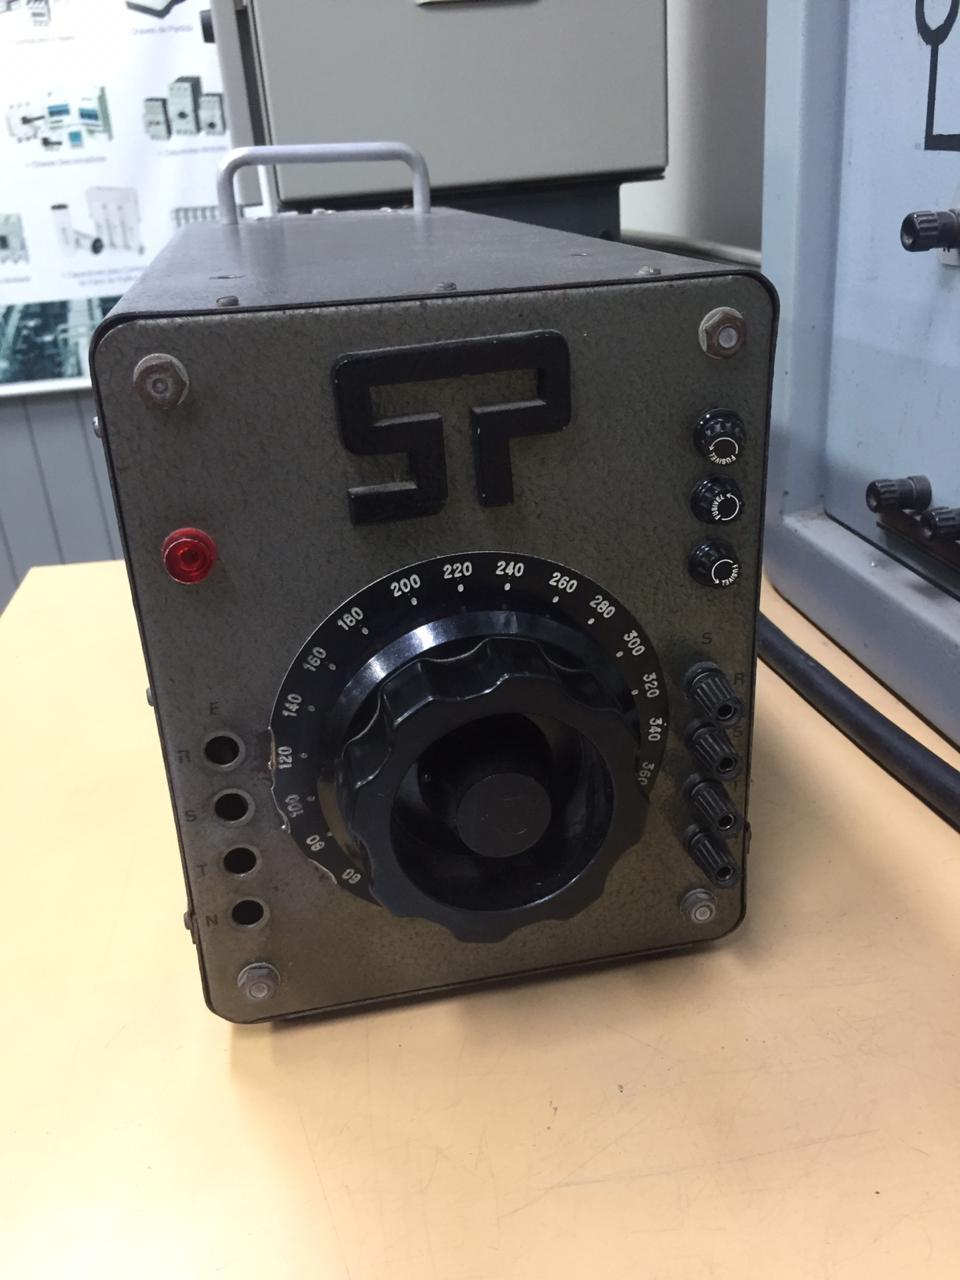
\includegraphics[width=5cm]{images/variac.jpeg}  
\caption{Variac.}
\label{variac} 
\end{figure}

\begin{figure}[h!]
\centering
    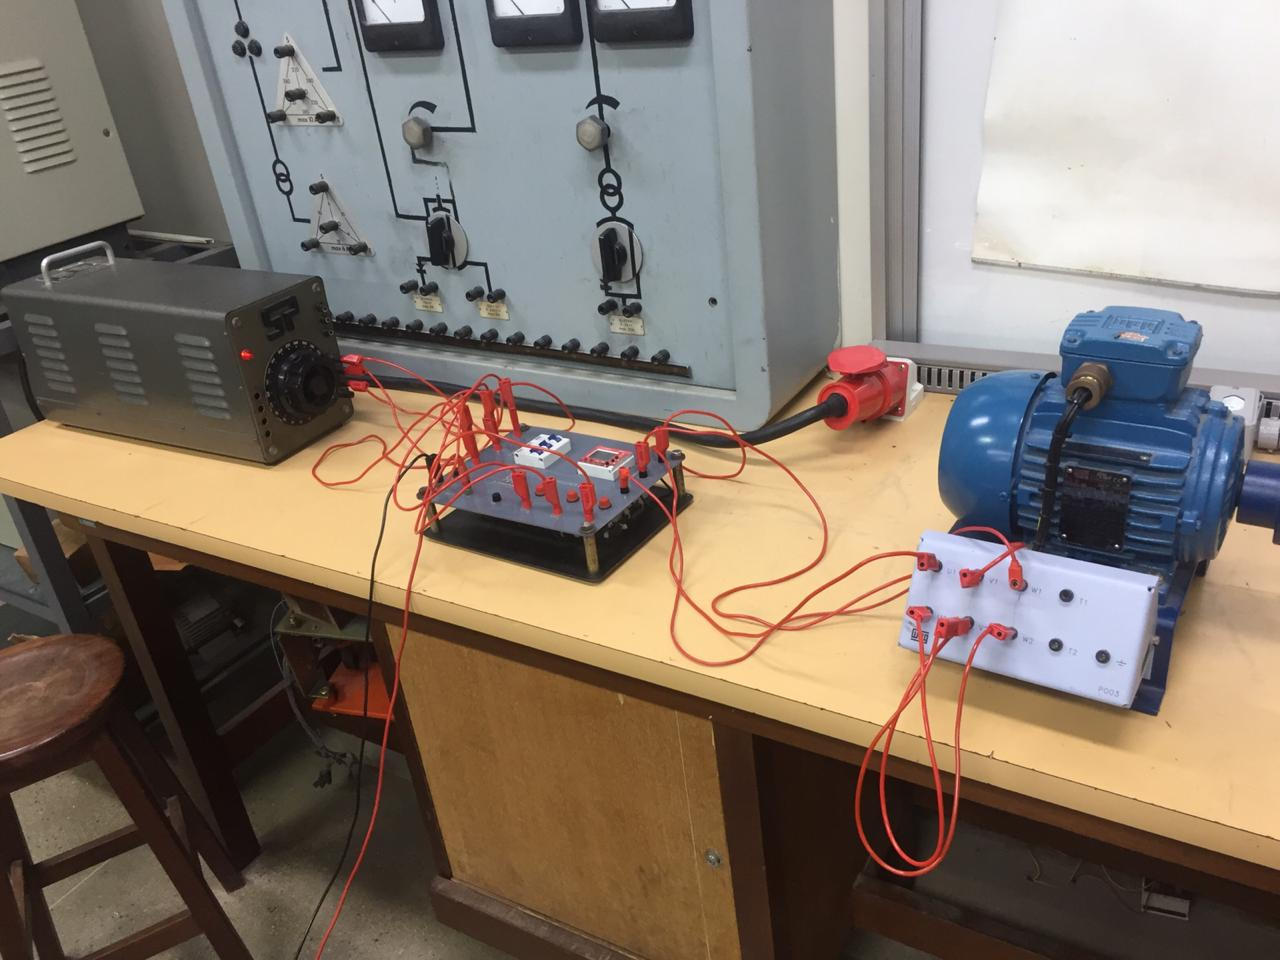
\includegraphics[width=9cm]{images/exp.jpeg}  
\caption{Experimento montado.}
\label{pratica} 
\end{figure}

 Após isso, as fases do variac passavam por um multimedidor, onde eram medidas as tensões, correntes e também as perdas, e após isso chegavam na máquina, onde foram os enrolamentos do estator foi ligado em Y, de forma a ficar na disposição desejada.

A maior diferença entre os dois ensaios é, claro, a disposição do rotor, implicando na alteração dos circuitos equivalentes. No motor de indução com rotor em vazio basta apenas dar partida no motor sem carga mecânica acoplada ao eixo até que a tensão seja a tensão nominal de 380V. Já para o ensaio com rotor bloqueado, um dos componentes do grupo segurou o rotor com mão, após o rotor devidamente travado, ajustou o variac de forma a fornecer 2.56A.

Durante os ensaios, anotou-se os valores de corrente, tensão e de potência com o multimedidor. Onde foi tudo auxiliado pelo Professor da disciplina e o técnico de laboratório, garantindo todos os cuidados necessários para não ter erros nas medições, nem problemas com os discentes ou com as próprias máquinas.

Após terminado os dois ensaios, usou-se um multímetro na opção de ohmímetro para medir os valores das resistências dos enrolamentos do estator da máquina.



\begin{figure}[h!]
\centering
    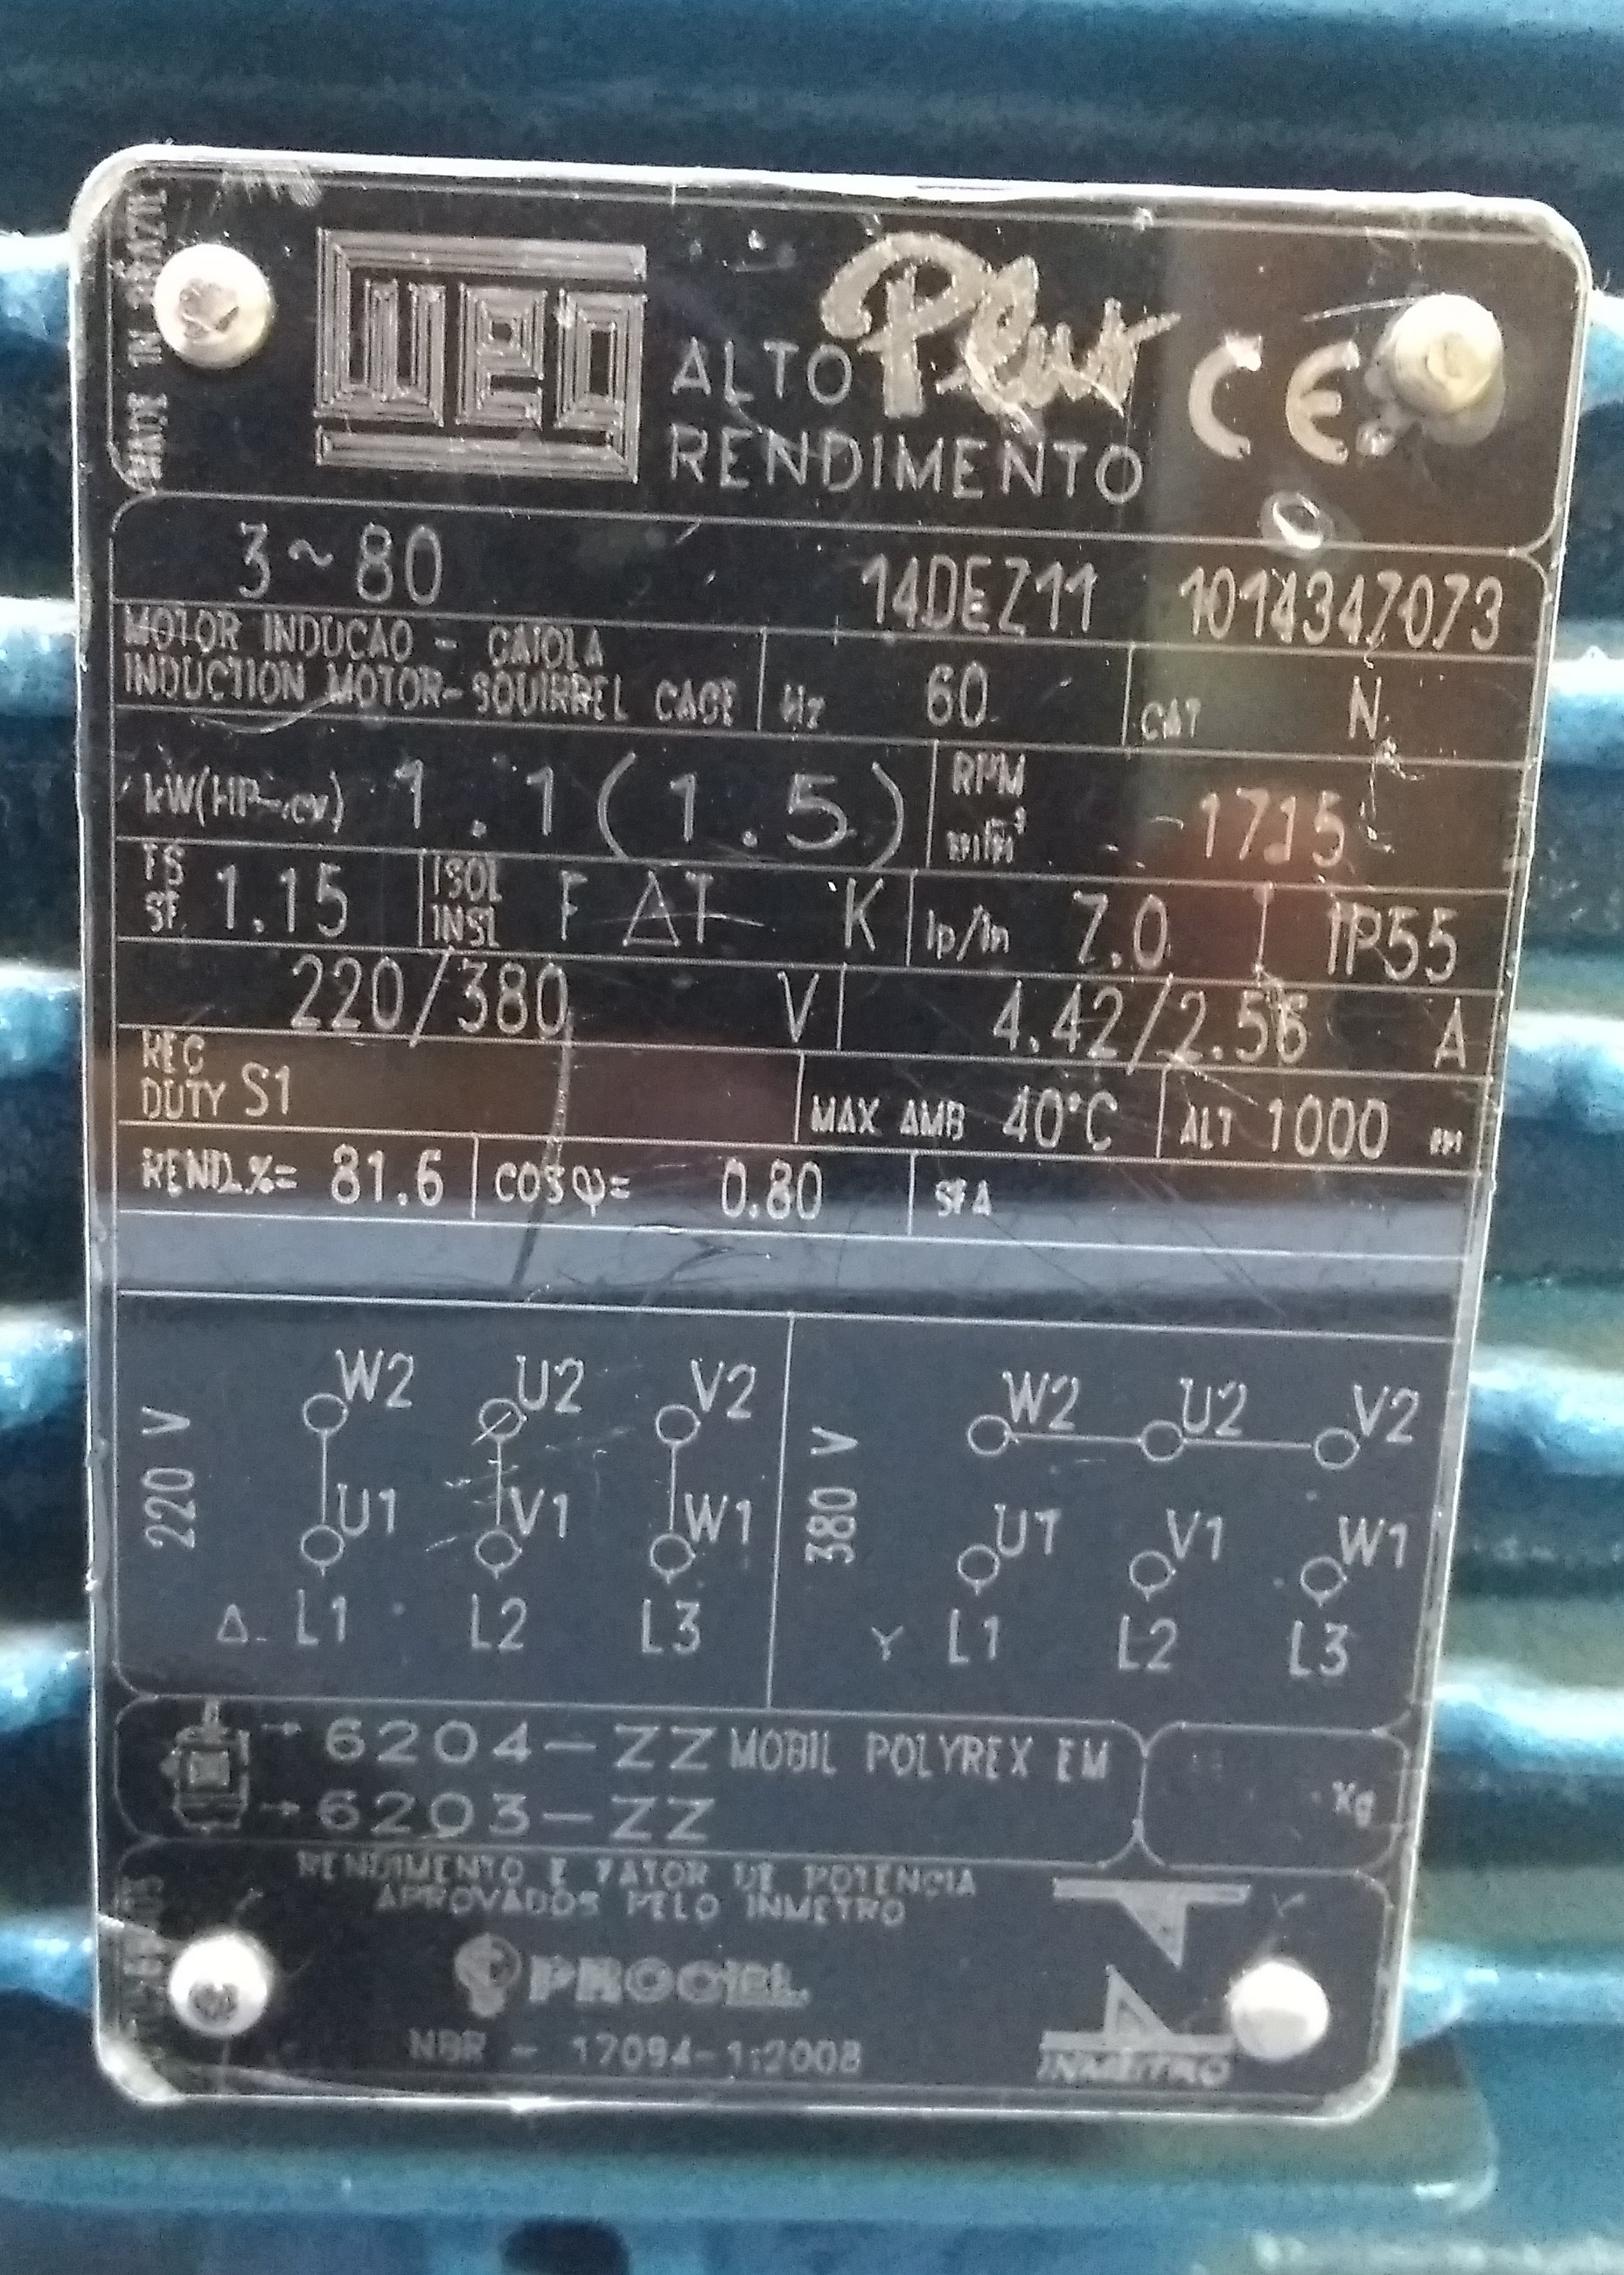
\includegraphics[width=7cm]{images/placa.jpg}  
\caption{Placa do motor utilizado. Contém a tensão de linha de 380V para ligação em estrela e 220V para ligação em triângulo; Fator de potência de 0.8 indutivo e rendimento de 81.6\%; Potência de 1.1kW; Corrente nominal para estrela de 2.56A e de 4.42A para triângulo; Rotação em potência nominal de 1715 rpm.}
\label{placa} 
\end{figure}



\pagebreak
